\section{Flowcharts}
\label{appendix:flowcharts}
% \begin{figure}
%     \caption{A flowchart of the TC receiving a sign request. Blue (dotted) nodes are only relevant in the first protocol.}
% \end{figure}

%\begin{table}
\renewcommand{\arraystretch}{1.1}
  \centering
  % \resizebox{\columnwidth}{!}{

    \begin{tabular}{ | c | l | }
      \hline
      Variable        & Description\\
    \hline
    \hline
    \multicolumn{2}{|l|}{\textit{Core parameters}} \\
    \hline
    \paramteff       & Effective revocation time\\
    \hline
    \paramtprl       & Minimum time in \acs{PRL} for safe revocation  \\
    \hline
    \multicolumn{2}{|l|}{\textit{Time parameters}} \\
    \hline
    \paramtt        & Validity period for timestamps  \\
    \hline
    $t$             & Current time at \acs{RA} \\
    \hline
    \funcnow        & Current \acs{TC} time \\
    \hline
    \paramtvv       & Timestamp sent in a \acs{V2V} message   \\
    \hline
    \paramthb       & Timestamp sent in a \ac{HB}   \\
    \hline
    \paramtrev        & Time of revocation issued by the \acs{RA}   \\
    \hline
    $t_{\mathrm{rcv}}$  & Time \acs{TC} receives message with revoked pseudonym  \\
    \hline
    % \paramtra         &    \\
    % \hline
    % \multicolumn{2}{|l|}{\textit{Attackers}} \\
    % \hline
    % \attackerhonest       &    \\
    % \hline
    % \attackersmart        &    \\
    % \hline
    % \attackersmarter        &    \\
    % \hline
    % \attackerblind        &    \\
    % \hline
  \end{tabular}
  % }
  \vspace{0.2cm}
  \caption{ List of all variables utilized in our design. }
  \label{tbl:eval-variables}
  %\vspace{-5mm}
\end{table}
%




\begin{figure}
    \begin{subfigure}[T]{.4\columnwidth}
        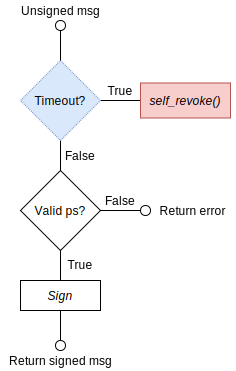
\includegraphics[width=\columnwidth]{figures/drawio/flowchart-sign.drawio.pdf}
    \end{subfigure}
    \unskip\ \vrule\
    \begin{subfigure}[T]{.4\columnwidth}
        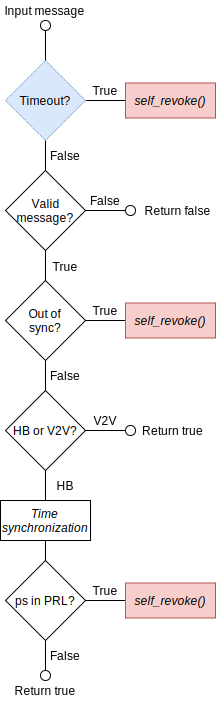
\includegraphics[width=\columnwidth]{figures/drawio/flowchart-process.drawio.pdf}
    \end{subfigure}
    \begin{minipage}{.45\columnwidth}
        \leavevmode\subcaption{Receiving a sign request.}
        \label{fig:appendix:flowchart-sign}
    \end{minipage}\hfil
    \begin{minipage}{.45\columnwidth}
        \leavevmode\subcaption{Receiving a message.}
        \label{fig:appendix:flowchart-process}
    \end{minipage}
    \caption{Flowcharts of the \acs{TC} logic. Blue (dotted) nodes are only
    relevant when a local trusted time source is available in \acsp{TC}.}
    \label{fig:appendix:flowchart}
\end{figure}

%Table~\ref{tbl:eval-variables} describes all variables used in the main paper
%for the reader's convenience. 
\cref{fig:appendix:flowchart} depicts flowcharts for the \ac{TC} behavior
described in our design. In particular, \cref{fig:appendix:flowchart-sign}
illustrates the steps taken to sign a \ac{V2V} message, while
\cref{fig:appendix:flowchart-process} shows the logic to verify a network
message, which can be either a \ac{HB} or a \ac{V2V} message.

According to \cref{req:v2v-receive,eq:valid-v2v-generic,eq:valid-heartbeat},
external messages should be verified with respect to authenticity (via digital
signature verification) and freshness (according to the validity window
\paramtt). Furthermore, the \ac{TC} should automatically perform self-revocation
if it detects de-synchronization (\cref{eq:auto-rev}). For every valid \ac{HB},
the \ac{TC} should synchronize its internal time \funcnow{}
((\cref{eq:time-update}), redundant if a local trusted time source is used), and
then inspect the \ac{PRL} to check whether self-revocation should be executed or
not (\cref{eq:self-rev}). For signing a message, the \ac{TC} should possess
valid pseudonyms in order to make a signature, which includes the input message
and context metadata such as timestamps (\cref{req:v2v-send}).

In \cref{fig:appendix:flowchart}, the \emph{timeout} condition in blue only
applies to the extension that takes into account a local trusted time source in
\ac{TC}, and checks if the current time is bigger than the biggest timestamp
received in a \ac{HB} plus \paramtt{} (\cref{eq:auto-rev-timeout}).